\section{Versuchsaufbau}
\label{sec:Versuchsaufbau}

Der Versuchsaufbau besteht aus einem Ultraschallteleskop,
zwei Ultraschallsonden und einem Rechner.\\
Die zwei Ultraschallsonden haben unterschiedliche Frequenzen.
Die eine Sonde hat eine Frequenz von $1 \, \si{\mega\hertz}$ und die andere
eine Frequenz von $2 \, \si{\mega\hertz}$.\\
Das Ultraschallteleskop wird ausschließlich im Echo-Impuls-Modus
verwendet. Mit einem Kippschalter kann allerdings zwischen dem
Echo-Impuls-Modus und dem Durchschallungs-Modus gewechselt werden. 
Da die zwei vorhandenen Sonden jedoch eine unterschiedliche Frequenz 
aufweisen, kann das Durchschallungsverfahren nicht angewandt werden.
Hier müssen Sender- und Empfängersonde die gleiche Frequenz haben.\\
Die Sendeleistung der Sonde kann mithilfe des Ultraschallteleskops 
in einem Bereich von $0$ bis $30 \, \si{\dB}$ eingestellt werden.\\
Der Rechner besitzt ein Programm zum Aufzeichnen und graphischen Interpretieren
der durch die Sonde empfangenen Impulse.\\
Da Luft eine große akustische Impedanz aufweist, wird als Kontaktmittel
zwischen Sonde und zu untersuchenden Objekt bidestilliertes Wasser
verwendet.\\


\section{Durchführung}
\label{sec:Durchführung}

Die Versuchsreihe besteht aus insgesamt vier Teilversuchen. Als erstes wird
ein Acrylblock mittels A-Scan untersucht.\\

\subsection{Untersuchung eines Acrylblocks mit dem A-Scan}

Gegeben ist ein Acrylblock mit elf unterschiedlich großen Löchern.
Dieser Block wird für ein weiteres Vorgehen zunächst mit einer Schieblehre
vermessen.\\
Anschließend wird mittels A-Scan die Schallgeschwindigkeit in dem 
Acrylblock untersucht, indem mit der Sonde sieben ausgewählte Löcher
durchschallt werden und die Laufzeit bestimmt wird.\\
Anhand der vorher
ausgemessenen Daten für die Lage der Löcher kann die Schallgeschwindigkeit
bestimmt werden. Es wird hierfür die $2 \, \si{\mega\hertz}$ Sonde verwendet.\\
Aufgrund der Anpassungsschicht der Sonde weist die Schallgeschwindigkeit eine
systematische Abweichung auf, welche mithilfe einer Ausgleichsrechnung
bestimmt werden kann.\\
Anschließend werden mittels A-Scan die Lage und Größe aller elf Bohrungen
untersucht. Dafür werden zunächst alle Bohrungen durchschallt und Laufzeiten
notiert. Dann wird der Block umgedreht und erneut durchschallt und Laufzeiten 
aufgezeichnet.\\
Der verwendete Acrylblock ist in einer Frontalskizze in \autoref{Abb:Acrylblock} zu sehen.

\begin{figure}
    \centering
    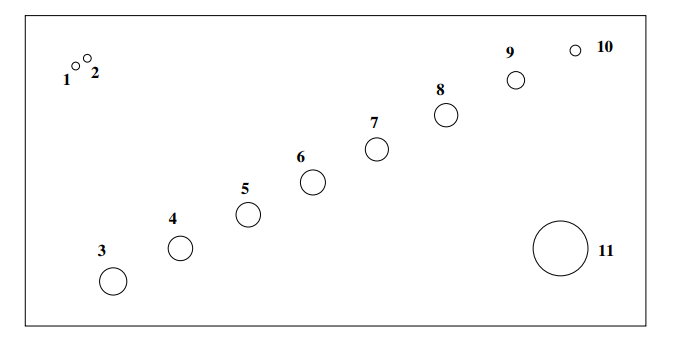
\includegraphics[width=0.5\textwidth]{messwerte/Acrylblock.png}
    \caption{Frontalskizze des verwendeten Acrylblocks.}
    \label{Abb:Acrylblock}
\end{figure}

\subsection{Untersuchung des Auflösungsvermögens}

In dem Acrylblock sind zwei kleine benachbarte Stellen (Loch eins und zwei).
Diese zwei Bohrungen sollen mittels A-Scan weitergehend untersucht werden.\\
Es wird die $1 \, \si{\mega\hertz}$ und die $2 \, \si{\mega\hertz}$
Sonde verwendet.\\
Es werden beide Aufnahmen mittels der graphischen Interpretation
des Rechners auf ihre Auflösung und Dämpfung hin untersucht.\\

\subsection{Untersuchung eines Acrylblocks mit dem B-Scan}

In diesem Versuchsteil werden wie bei den vorherigen Versuchen
die Bohrungen des Acrylblocks untersucht. Dies wird jedoch
diesmal mittels B-Scan durchgeführt.\\
Es wird die $2 \, \si{\mega\hertz}$ Sonde angeschlossen und ein
Laufscan über mehrere Sekunden von links nach rechts aufgenommen 
und in einem zweidimensionalen Bild gespeichert. Dieses Bild wird 
durch den Rechner automatisch erzeugt.\\
Der Acrylblock wird nun umgedreht und obiges Verfahren erneut
angewendet.\\
Es werden die Abmessungen der Störstellen ermittelt und mit den
vorherigen Ergebnissen verglichen.\\

\subsection{Untersuchung eines Brustmodells mit einem B-Scan}

In diesem Versuchsteil steht ein Brustmodell zur Verfügung.
In diesem Modell stecken zwei Tumore. Ein Tumor ist mit Flüssigkeit gefüllt (auch Zyste genannt)
und einer besteht aus festen Gewebe.\\
Per Abtasten werden die groben Positionen der Tumore bestimmt und 
anschließend mittels A-Scan und der $2 \, \si{\mega\hertz}$ Sonde
untersucht.\\
Danach werden mehrere B-Scans entlang gedachter Linien
aufgenommen bis die zwei Tumore gut sichtbar sind.\\
Anhand dieser Aufnahmen wird nun Größe und Lage der Tumore bestimmt.\\